\documentclass[11pt,a4paper]{article}

\usepackage[utf8]{inputenc}
\usepackage[T1]{fontenc}
\usepackage[spanish,es-tabla]{babel}
\usepackage{lmodern}
\usepackage[margin=2.5cm]{geometry}
\usepackage{graphicx}
\usepackage{booktabs}
\usepackage{tabularx}
\usepackage{array}
\usepackage{amsmath}
\usepackage{enumitem}
\usepackage{caption}
\usepackage{float}
\usepackage{needspace}
\usepackage{tikz}
\usetikzlibrary{arrows.meta,babel}
\definecolor{radar}{RGB}{37,99,235}
\definecolor{agua}{RGB}{16,150,120}
\usepackage[hidelinks]{hyperref}

\graphicspath{{figuras/}}
\newcolumntype{L}{>{\raggedright\arraybackslash}X}
\setlength{\parskip}{0.5em}
\setlength{\parindent}{0pt}
\renewcommand{\arraystretch}{1.3}

\begin{document}

% ======================================================
% PORTADA
% ======================================================
\begin{titlepage}
    \centering
    {\large Universidad Nacional de Asunción\par}
    {\large Facultad de Ingeniería\par}
    {\large Carrera de Ingeniería Mecatrónica\par}
    \vspace{1.2cm}
    
\includegraphics[width=0.32\textwidth]{logo_fiuna.png}\par
    \vspace{1.2cm}
    {\Large Proyecto 4\par}
    \vspace{1.2cm}
    {\LARGE\bfseries Sistema de adquisición y monitoreo\\de nivel de agua\par}
    \vspace{0.6cm}
    {\Large Informe de puntos de mejora y alcance\par}
    \vfill
    \begin{flushleft}
        \textbf{Profesores:}\\
        Prof. Ing. Federico Gaona, MSc.\\
        Prof. Ing. Esteban Fretes\\[1em]
        \textbf{Alumnos:}\\
        \begin{tabular}{@{}ll}
            Héctor Dejesús Velázquez Ojeda   & 5.011.166 \\
            Mathias Ramón Aguilar DelValle   & 4.970.804 \\
            Mauricio Iván Tullo Estigarribia & 3.782.101 \\
        \end{tabular}
    \end{flushleft}
    \vspace{1cm}
    {\large San Lorenzo, Paraguay\par}
    {\large 2026\par}
\end{titlepage}

% ======================================================
% 1. RESUMEN
% ======================================================
\section{Resumen}

La primera entrega obtuvo \textbf{46/50} y en la planilla de evaluación quedó
(71/100). Los criterios más bajos fueron validación (2,5/5)
y objetivos (3/5).

Este informe se concentra en esos dos puntos. Para la validación cambiamos a un
sensor radar más exacto y planificamos ensayos con resultados medibles; para los
objetivos, los reducimos de 15 a 5, cada uno con su criterio de verificación.

% ======================================================
% 2. NUEVO SENSOR
% ======================================================
\section{Nuevo sensor: radar de 80 GHz}

Reemplazamos el sensor ultrasónico por un radar (Luda / POLIVIR, modelo FM02B)
con exactitud de \textbf{$\pm$3 mm}. Además del nivel mide la velocidad
superficial del agua.

\begin{figure}[H]
    \centering
    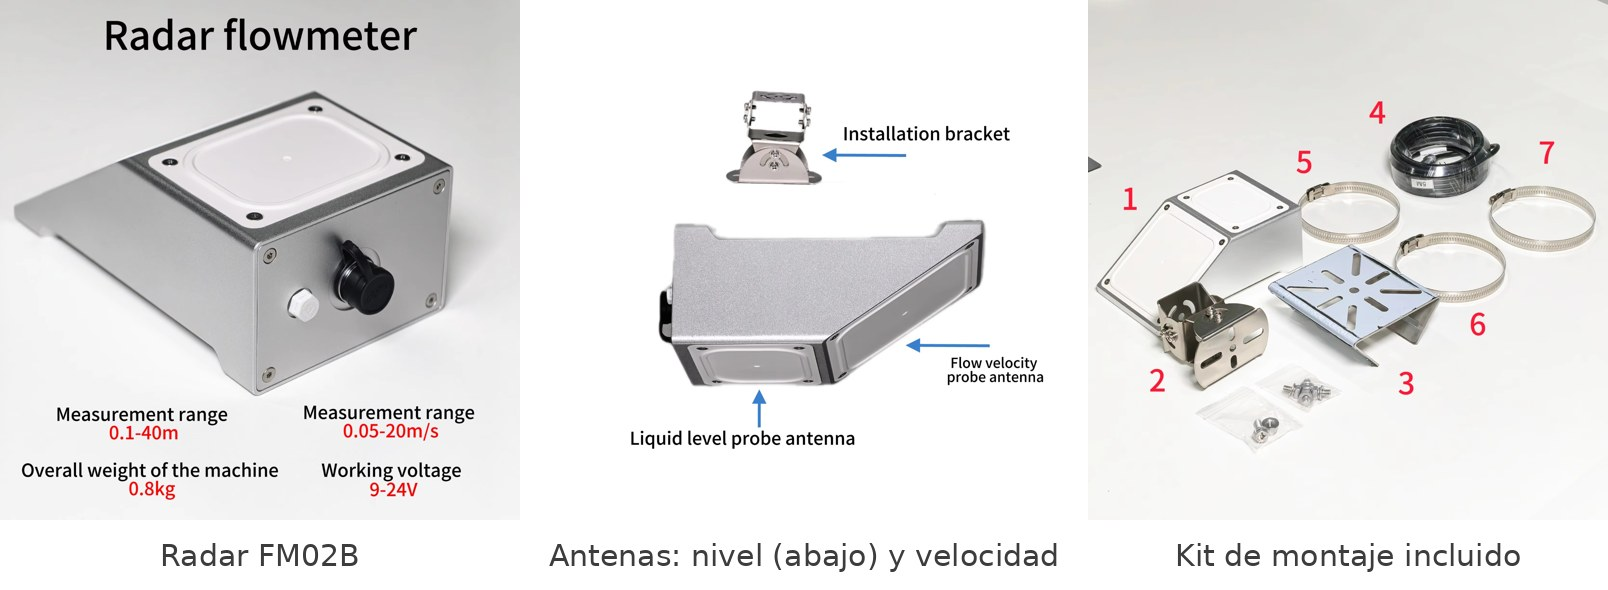
\includegraphics[width=\textwidth]{sensor_fotos.jpg}
    \caption{Radar FM02B, sus antenas y kit de montaje.}
\end{figure}

\begin{table}[H]
    \centering
    \caption{Datos principales del radar.}
    \begin{tabular}{ll}
        \toprule
        \textbf{Dato} & \textbf{Valor} \\
        \midrule
        Rango de nivel          & 0,1 -- 40 m \\
        Exactitud / resolución  & $\pm$3 mm / 1 mm \\
        Haz de la antena        & 14° \\
        Alimentación            & 12 V, hasta 160 mA \\
        Comunicación            & RS485 a 115200 baudios \\
        \bottomrule
    \end{tabular}
\end{table}

El kit trae soporte orientable, placa para poste, abrazaderas inoxidables y
5 m de cable. Con él, la parte mecánica se reduce al montaje del sensor.

% ======================================================
% 3. VALIDACION
% ======================================================
\needspace{9\baselineskip}
\section{Validación: qué probamos en P3 y qué falta}

En Proyecto 3 cada prueba se informó como \emph{correcta}, con video como
evidencia. La planilla pide resultados medibles, así que partimos de esas
pruebas y les agregamos números.

\begin{table}[H]
    \centering
    \caption{Pruebas de P3 y lo que falta cuantificar.}
    \begin{tabularx}{\textwidth}{>{\raggedright\arraybackslash}p{3.0cm}LL}
        \toprule
        \textbf{Prueba} & \textbf{Evidencia de P3} & \textbf{Qué falta medir} \\
        \midrule
        Medición de nivel & Lecturas válidas del sensor en banco (video). &
            Error en mm frente a cinta métrica, ya con el radar nuevo. \\
        Store and Forward & Dato pendiente reenviado al volver la conexión
            (video). & Datos perdidos y duplicados en $\geq$ 10 cortes de red y
            energía; tiempo de recuperación. \\
        Operación en campo & Unos 9 meses de datos en el arroyo, vistos en
            Grafana. & Porcentaje de disponibilidad y huecos calculados a
            partir de esos datos. \\
        Alimentación & Sistema funcionando con la mini UPS. & Consumo por
            módulo y autonomía ante un corte de energía. \\
        \bottomrule
    \end{tabularx}
\end{table}

% ======================================================
% 4. PUNTOS DE MEJORA
% ======================================================
\needspace{9\baselineskip}
\section{Puntos de mejora}

Agrupamos las observaciones de la planilla en 6 áreas. Cada tarjeta indica qué
faltaba y qué haremos para la próxima entrega.

\begin{figure}[H]
    \centering
    \resizebox{0.92\textwidth}{!}{% Diagrama: seis areas a mejorar; la validacion es la mas debil
\newcommand{\tarjeta}[6]{%
    % #1 estilo, #2 area, #3 puntaje, #4 faltaba, #5 accion 1, #6 accion 2
    \begin{minipage}[t][2.05cm][t]{7.1cm}
        \textbf{#2}\hfill#3\\[2pt]
        {\footnotesize\color{gray!60!black} Faltaba: #4}\\[3pt]
        {\footnotesize\textbullet\ #5\\[1pt]\textbullet\ #6}
    \end{minipage}%
}
\begin{tikzpicture}[
    card/.style={draw=gray!60, thick, rounded corners=4pt, inner sep=7pt, anchor=north west},
    destacada/.style={card, draw=radar, very thick, fill=radar!10}
]
    \node[destacada] at (0,0) {\tarjeta{}{Validación y seguridad}{\textbf{2,5/5}}
        {probar pérdida de datos y exactitud}
        {Cortes de red y energía: enviados vs.\ recibidos}
        {Calibrar el radar en banco a 5 distancias}};
    \node[card] at (7.75,0) {\tarjeta{}{Electrónica y firmware}{4/5}
        {consumo, autonomía y SD ante cortes}
        {Medir consumo y calcular autonomía (UPS)}
        {Trama con ID, hora UTC y estado; sin $-1$}};
    \node[card] at (0,-2.75) {\tarjeta{}{Mecánica: montaje del sensor}{3,5/5}
        {definir el montaje del sensor}
        {Montaje del radar con su kit de soporte}
        {Antena nivelada y haz de 14° sin obstáculos}};
    \node[card] at (7.75,-2.75) {\tarjeta{}{Interfaz}{4/5}
        {aviso de dato viejo o inválido}
        {Mostrar antigüedad del dato y estado del sensor}
        {Alarma si dejan de llegar datos}};
    \node[card] at (0,-5.5) {\tarjeta{}{Objetivos y metodología}{3/5}
        {15 objetivos que eran actividades}
        {5 objetivos medibles, uno por área}
        {Fases: requisitos, sensor, ensayos en laboratorio}};
    \node[card] at (7.75,-5.5) {\tarjeta{}{Documentación y bibliografía}{3,5/5}
        {ficha del sensor, costos, línea base}
        {Citar fabricante; comparar 3 tipos de sensor}
        {Costos completos y datos de 9 meses de uso}};
\end{tikzpicture}
}
    \caption{Puntos de mejora por área y puntaje de la planilla.}
\end{figure}

% ======================================================
% 5. FUERA DE ALCANCE
% ======================================================
\needspace{9\baselineskip}
\section{Fuera de alcance}

Estos puntos no se harán completos en Proyecto 4; quedan documentados como
límites.

\begin{table}[H]
    \centering
    \caption{Puntos fuera de alcance y su justificación.}
    \begin{tabularx}{\textwidth}{>{\raggedright\arraybackslash}p{4.2cm}L}
        \toprule
        \textbf{Punto} & \textbf{Por qué queda fuera} \\
        \midrule
        Montaje del sensor en el arroyo & La instalación en el sitio depende
            del Departamento de Mecánica y Energía y del grupo de investigación
            Mburicaó. Para la presentación montamos el radar en un banco de
            laboratorio que simula la instalación. \\
        Medir caudal & Requiere relevar la sección del cauce y calibración
            hidráulica. Solo registramos la velocidad como dato extra. \\
        Calibrar en todo el rango (0,1--40 m) & El arroyo no permite fijar
            niveles. Calibramos en banco de laboratorio a distancias conocidas. \\
        Usuarios y permisos en la web & La página es pública y solo muestra
            datos; no hay comandos que proteger. \\
        Validar la predicción con IA & Es parte del proyecto de investigación
            Mburicaó, no de este trabajo; solo se cita. \\
        Panel solar & El sitio tiene red eléctrica y la UPS cubre los cortes. \\
        \bottomrule
    \end{tabularx}
\end{table}

% ======================================================
% 6. OBJETIVOS REFORMULADOS
% ======================================================
\needspace{9\baselineskip}
\section{Objetivos reformulados}

Pasamos de 15 objetivos a 5, uno por área, manteniendo los que el profesor
marcó como correctos (1, 8, 10, 11 y 13). Los criterios de aceptación son
propuestas a confirmar antes de ensayar.

\textbf{Objetivo general:} diseñar y validar una estación que mida y transmita
el nivel del arroyo Mburicaó, con el sensor correctamente montado y una
interfaz que muestre datos confiables y avise de fallas.

\begin{table}[H]
    \centering
    \caption{Objetivos específicos y cómo se verifican.}
    \begin{tabularx}{\textwidth}{>{\raggedright\arraybackslash}p{2.2cm}LL}
        \toprule
        \textbf{Área} & \textbf{Objetivo} & \textbf{Cómo lo verificamos} \\
        \midrule
        Electrónica & Integrar radar, RTC, microSD y módem en la PCB, con
            consumo y autonomía calculados. & Consumo medido por módulo y
            autonomía con la UPS. \\
        Firmware & Enviar datos sin perderlos ante cortes (Store and Forward
            con ID por dato). & 0 datos perdidos o duplicados tras $\geq$ 10
            cortes. \\
        Montaje del sensor & Montar el radar con su kit de soporte en un
            banco de laboratorio que simule la instalación, con la antena
            nivelada. & Lecturas
            estables con el radar montado; haz de 14° sin obstáculos. \\
        Interfaz & Mostrar históricos, antigüedad del dato, estado del sensor
            y alarma. & Capturas con dato válido, viejo y en falla. \\
        Validación & Medir la exactitud del nivel en el banco de laboratorio. &
            Error $\leq \pm$10 mm frente a cinta métrica. \\
        \bottomrule
    \end{tabularx}
\end{table}

\end{document}
